\documentclass[10pt,a4paper]{article}
\usepackage[utf8]{inputenc} 
% para poder usar tildes en archivos UTF-8 
\usepackage[spanish]{babel} 
% para que comandos como \today den el resultado en castellano 
\usepackage{a4wide} 
% márgenes un poco más anchos que lo usual 
\usepackage[conEntregas]{caratula}
\usepackage{makeidx}
\usepackage{graphicx}
\usepackage{grffile}
\usepackage{amsmath}
\usepackage{amssymb}

\begin{document}

\titulo{Trabájo Práctico 1} \subtitulo{Quake III FastInvSqrt()}

\fecha{\today}

\materia{Métodos Numéricos}
% \grupo{Grupo Los Amantes de tu Hermana}

\integrante{Escalante, José}{822/06}{joe.escalante@gmail.com}
\integrante{Raskovsky, Iván Alejandro}{57/07}{iraskovsky@dc.uba.ar}
\integrante{Osinski, Andrés}{405/07}{andres.osinski@gmail.com}

% TODO: Agregar abstract y 4 palabras claves

% El tutulo debera ser breve y apropiado para una rapida identificacion del
% contenido del trabajo. El resumen, de no mas de 200 palabras, debera explicar
% brevemente el trabajo realizado y las conclusiones de los autores de manera
% que pueda ser util por ser solo para dar una idea del contenido del trabajo.
% Las palabras clave, no mas de cuatro, deben ser terminos tecnicos que den una
% idea del contenido del trabajo para facilitar su busqueda en una base de
% datos tematica.

\maketitle
\tableofcontents
\newpage

    \section{Abstract}

En este trabajo vamos a mostrar dos formas de poder
calcular la inversa de la raíz cuadrada, a partir de adaptar el problema a la
búsqueda de ceros de una función. Iremos documentando también los resultados
obtenidos a partir de ciertas familias de inputs elegidas con cierto
criterio.\\

En particular veremos el método de Newton y el de la Secante para llegar al
resultado mencionado\\

Los experimentos nos terminaron mostrando que el método de Newton termina
siendo mejor en cuestiones de orden de convergencia y error, y resulta evidentemente más conveniente utilizar $\beta$
que $\e$ para realizar los cálculos.\\

{\bf Palabras clave:}
\begin{itemize} 
    \item Método de Newton 
    \item Método de la Secante 
    \item Criterios de comparación 
\end{itemize}

    \newpage
    \section{Introducción Teórica}

Las funciones que usaremos para aproximar la inversa de la raíz son las siguientes:

\begin{displaymath}
    f(x) = x^2 - \alpha
\end{displaymath}

\begin{displaymath}
    e(x) = \frac{1}{x^2} - \alpha
\end{displaymath}

A partir de este momento nos enfocaremos en encontrar los ceros de estas dos funciones usando los métodos de Newton y de la Secante:

\begin{itemize}
    \item {\bf Newton:} $\displaystyle x_{n + 1} = x_n - \frac{h(x_n)}{h'(x_n)}$

    \item {\bf Secante:} $\displaystyle x_{n + 1} = x_{n - 1} - h(x_{n - 1})\frac{x_{n - 1} - x_{n - 2}}{h(x_{n - 1}) - h(x_{n - 2})}$
\end{itemize}

Donde $h(x) = f(x)$ o $h(x) = e(x)$ cuando corresponda 

\subsection{Análisis de $f(x)$}

Llamemos $\displaystyle \beta = \frac{1}{\alpha}$. Por otro lado la expresión de $f(x)$ la podemos reescribir de esta manera:

\begin{displaymath}
    f(x) = x^2 - \alpha = (x + \sqrt{\alpha})(x - \sqrt{\alpha})
\end{displaymath}

Estas raíces existen pues $\alpha > 0$ (pues no existe la raíz de un negativo en $\mathbb{R}$) y como podemos ver las raíces son iguales en módulo y nos sirven para hallar $\beta$ con la salvedad de que si obtenemos el valor negativo simplemente le cambiamos el signo. Por lo tanto si $\displaystyle x = \sqrt{\alpha} \implies \beta = \frac{1}{x}$

INSERTAR GRÁFICO DE f(x)

$f(x)$ es convexa y su derivada segundo es $f''(x) = 2$, al ser constante y por la
forma que tienen las derivadas asumimos que siempre va a converger.

\subsection{Análisis de $e(x)$}

\begin{displaymath}
    e(x) = 0 \implies 0 = \frac{1}{x^2} - \alpha \implies \alpha = \frac{1}{x^2} \implies x^2 = \frac{1}{\alpha}
\end{displaymath}

$e(x)$ con $\alpha > 0$ también tiene dos raíces por lo que al igual que con
$f(x)$ nos es indistinto cuál de las dos obtenemos. En este caso es importante
notar que en el 0, hay una asíntota de las ordenadas.\\

INSERTAR GRÁFICO DE e(x)
 
Los dos métodos que elegimos trabajan con la tangente de las funciones en un
punto o con una aproximación de esta.

Observamos $e''(x) = 6/x^4$. Esto quiere decir que la misma tiene una asíntota en el 0,
y una pendiente que se agudiza rápidamente cerca de 0, lo cual puede dificultar la convergencia,
dado que para que las operaciones aritméticas involucradas en los métodos de aproximación 
den resultados de buena precisión, dependen de trabajar con números bien representables en punto flotante.

\subsection{Prueba de la convergencia de Newton}
Vamos a demostrar inductivamente la convergencia del método de Newton usando la función $\displaystyle f(x) = x^2 - \alpha$. De esta manera la sucesión nos queda:

\begin{displaymath}
    x_{n + 1} = \frac{1}{2}(x_n + \frac{\alpha}{x_n})
\end{displaymath}

Lo que queremos demostrar es que si $x_0 > \sqrt{\alpha}$ entonces $x_{n + 1} < x_n$ para todo $n > 0$.\\

{\large \bf Inducción en k $\in \mathbb{N}$}\\
Queremos probar que $x_{k + 1} < x_k$.\\

{\bf Caso base: $P(0)$}\\
Sea $k = 1$, queremos ver que $x_1 < x_0$. Entonces reemplazando $x_1$ por su definición tenemos:

\begin{displaymath}
    \frac{1}{2}(x_0 + \frac{\alpha}{x_0}) < x_0 \iff x_0 + \frac{\alpha}{x_0} < 2x_0 \iff \frac{\alpha}{x_0} < x_0 \iff \alpha < x_0^2 \iff \sqrt{\alpha} < x_0
\end{displaymath}

Y esto último es la precondición. Por lo tanto $x_1 < x_0$ $_\square$\\

Veamos también que $x_1 > \sqrt{\alpha}$\\

\begin{displaymath}
    x_1 > \sqrt{\alpha} \iff \frac{1}{2}(x_0 + \frac{\alpha}{x_0}) > \sqrt{\alpha} \iff x_0 + \frac{\alpha}{x_0} > 2\sqrt{\alpha}
\end{displaymath}

\begin{displaymath}
    \iff x_0 - 2\sqrt{\alpha} > -\frac{\alpha}{x_0} \iff x_0^2 - 2\sqrt{\alpha}x_0 + \alpha > 0 \iff (x_0 - \sqrt{\alpha})^2 > 0
\end{displaymath}

Luego esto último vale pues $x_0 > \sqrt{\alpha}$. Por lo tanto, por esto y por lo demostrado antes vale que:

\begin{displaymath}
    \sqrt{\alpha} < x_1 < x_0
\end{displaymath}

{\bf Caso n + 1: $P(n) \implies P(n + 1)$}\\
Sea $k = n + 1$. Queremos probar que $x_{n + 1} < x_n$. Por lo visto en nuestro caso base la {\bf Hipótesis Inductiva} es:

\begin{displaymath}
    \sqrt{\alpha} < x_n < x_{n - 1}
\end{displaymath}

Entonces:
\begin{displaymath}
    x_{n + 1} = \frac{1}{2}(x_n + \frac{\alpha}{x_n}) = \frac{x_n^2 + \alpha}{2x_n}
\end{displaymath}

Luego por {\bf HI} vale que $\sqrt{\alpha} < x_n \iff \alpha < x_n^2 $ Entonces:

\begin{displaymath}
    \frac{x_n^2 + \alpha}{2x_n} < \frac{x_n^2 + x_n^2}{2x_n} = x_n
\end{displaymath}

Por lo tanto $x_{n + 1} < x_n$ $\square$

    \newpage
    % Deben explicarse los metodos numericos que utilizaron y su aplicacion al
% problema concreto involucrado en el trabajo practico. Se deben mencionar los
% pasos que si- guieron para implementar los algoritmos, las dicultades que
% fueron encontrando y la descripcion de como las fueron resolviendo. Explicar
% tambien como fueron planteadas y realizadas las mediciones experimentales.
% Los ensayos fallidos, hipotesis y conjeturas equivocadas, experimentos y
% metodos malogrados deben gurar en esta seccion, con una breve explicacion
% de los motivos de estas fallas (en caso de ser conocidas)

\section{Implementación}

Para realizar el análisis de los métodos y funciones previamente descriptos
realizamos una implementación en \verb|C| que nos permite decidir
paramétricamente cómo resolver la inversa de la raíz de un número dado.

La implementación acepta los siguientes parámetros:

\begin{itemize}
    \item Función $e(x)$ o $f(x)$
    \item Método de Newton o de la Secante
    \item Criterio de parada:
    \begin{itemize}
        \item Cantidad de iteraciones
        \item Tiempo de Ejecución
        \item Error Absoluto
        \item Error Relativo
    \end{itemize}
    \item Eleccion de $x_0$ y $x_1$ ($x_1$ solo para el método de la Secante)
\end{itemize}

Luego de obtenido el resultado en base a los parámetros elegidos nuestra
implementación devuelve:

\begin{itemize}
    \item la aproximación en cada iteración
    \item el error absoluto
    \item el error relativo
    \item el tiempo de ejecución
\end{itemize}

Realizamos también unos helpers en \verb|Python| para poder crear experimentos
de forma sencilla, poder replicarlos cuantas veces sea necesario y analizar
los resultados.

El código escrito se puede optimizar \textbf{mucho}, sobre todo en las cuentas
que realiza el cuerpo de cada metodo. Ahora hay una implementación naive que
replica el enfoque analítico pero que a nivel cantidad y complejidad de
operaciones se puede mejorar.

Por otro lado, hay un alto grado de overhead debido a la forma que decidimos
implementar la flexibilidad de ejecución con los parámetros elegidos, pero
podemos ver que esto afecta a los dos métodos y funciones por igual por lo que
no debería afectar las comparaciones y resultados.

\newpage
\section{Desarrollo}

Decidimos analizar las siguientes combinaciones entre métodos y funciones para
calcular la inversa de la raíz de un número:

\begin{itemize}
    \item raíz de $f(x)$ aproximada mediante el método de Newton
    \item raíz de $e(x)$ aproximada mediante el método de Newton
    \item raíz de $e(x)$ aproximada mediante el método de la Secante
\end{itemize}

Recordemos que para el caso de estas funciones, es lo mismo encontrar
cualquiera de sus raices ya que tienen igual módulo y encontrando una raíz se
puede encontrar la otra cambiando el signo (\ref{sec:analisis_f_x}
y~\ref{sec:analisis_e_x}).

\subsection{Ajuste de parámetros}\label{sec:ajuste_parametros}

Cada una de estas variantes tiene parámetros según el método utilizado que se
pueden ajustar según la función a analizar. En particular para el método de
Newton hay que elegir una primera aproximación $x_0$ en base a $f(x)$ o $e(x)$
(que puede o no ser la misma) y para el método de la Secante y $e(x)$ hay que
elegir $x_0$ y $x_1$.

Decidimos realizar nuestro análisis enfocados en una amplia gama de magnitudes
de números a los cuales les queremos buscar la inversa de la raíz. Estamos
interesados tanto en números muy pequeños, cercanos al cero y en números muy
grandes, lejanos del 0.

Por esta razón, para el ajuste de parámetros decidimos utilizar un criterio de
parada de error relativo entre iteraciones. Gracias a esta elección y el
caracter iterativo de los métodos a utilizar nos garantizamos que no importa la
magnitud del número dado, siempre encontraremos una solución con un error
relativo al resultado pequeño, por lo que los parámetros a elegir nos deben
otorgar buenos resultados para números muy grandes y muy pequeños.

\subsubsection{Ajuste de $x_0$ para $f(x)$ y el método de Newton}
\label{ssub:ajuste_f_x0_newton}

Al buscar una raíz de $f(x)$ mediante el método de Newton tenemos asegurada la
convergencia para cualquier $x_0$ mayor a alguna de las raices
(\ref{sec:convergencia}). Al saber que existen dos raíces de igual módulo
podemos elegir $x_0 = 0 + \epsilon$ y tener garantizada la convergencia. Notar
que no se puede elegir $x_0 = 0$ ya que la recta tangente en ese punto es
constante y no se interseca con el eje de las abscisas. No obstante un análsis
analítico nos puede permitir elegir un mejor $x_0$.

\begin{figure}[!htbp]
  \begin{center}
    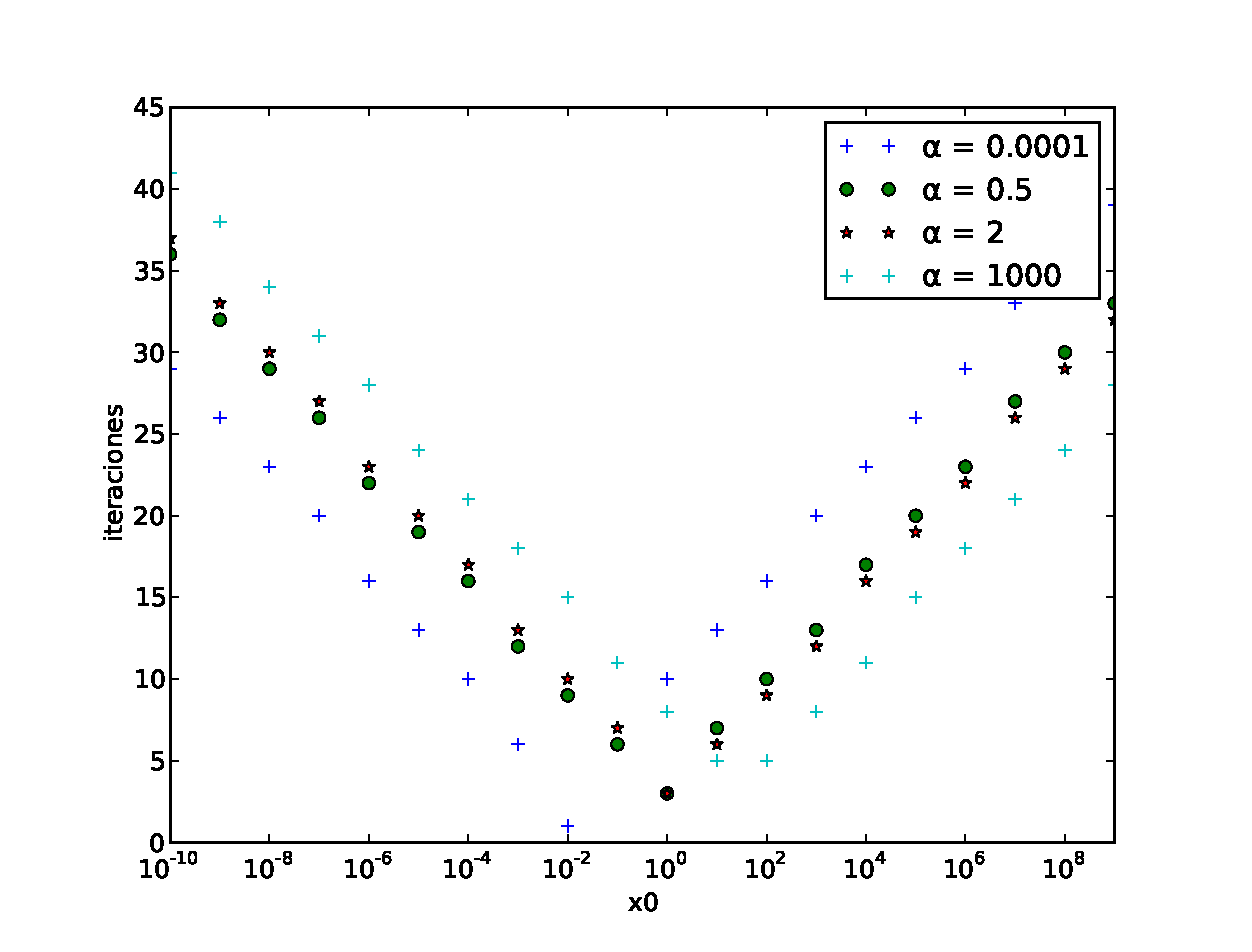
\includegraphics[scale=0.5]{graficos/new/f_newton_x0_variable.eps}
    \caption{\label{fig:f_newton_x0_variable} Gráfico de cantidad de iteraciones fijando $\alpha$ variando $x_0$ para $f(x)$ utilizando el método de Newton.}
  \end{center}
\end{figure}

En la Figura~\ref{fig:f_newton_x0_variable}  podemos ver como varía la cantidad
de iteraciones, cambiando la magnitud de $x_0$. Cuando $x_0$ es muy grande
empezamos muy lejos de la solución, con lo cual se requieren muchas iteraciones
para llegar al resultado.

Cuando $x_0$ es muy pequeño, cercano al $0$, la pendiente de la tangente a
$f(x)$ es cercana al 0, por lo que en la siguiente iteración $x_1$, el punto donde
esta recta se interseca con el eje de las abscisas es muy grande, cayendo en el
caso anterior partiendo desde $x_1$ de un punto muy grande, con un valor muy
alejado de la solución.

\begin{figure}[!htbp]
  \begin{center}
    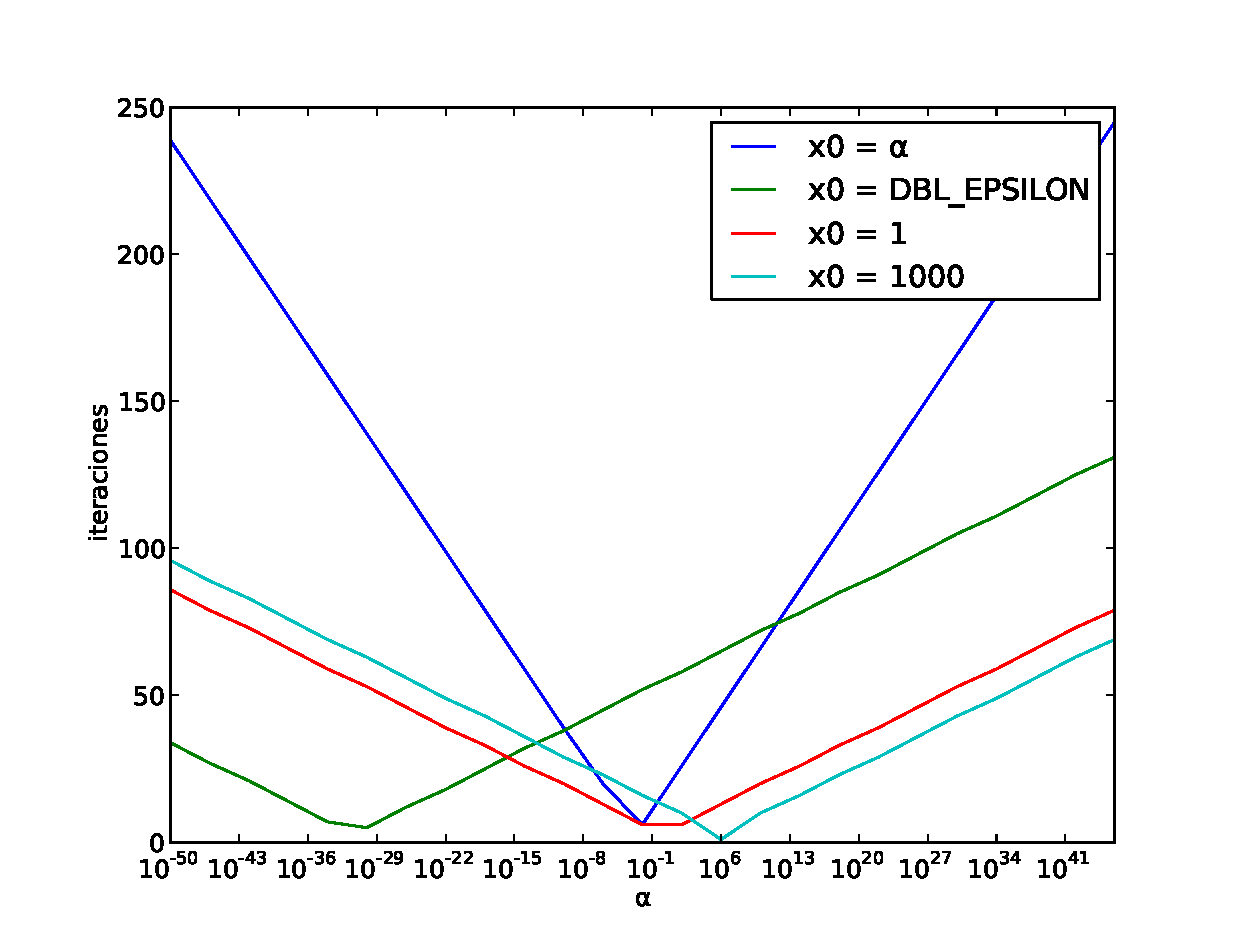
\includegraphics[scale=0.5]{graficos/new/f_newton_x0_fijo_1.eps}
    \caption{\label{fig:f_newton_x0_fijo_1} Gráfico de cantidad de iteraciones fijando $x_0$ variando $\alpha$ para $f(x)$ utilizando el método de Newton.}
  \end{center}
\end{figure}

En la Figura~\ref{fig:f_newton_x0_fijo_1} graficamos la cantidad de iteraciones
necesarias para llegar al resultado, fijando diferentes puntos de partida $x_0$
y variando la magnitud de $\alpha$. Las variantes que mostramos en esta figura
son $x_0$ constantes y en función del $\alpha$. Una de las opciones de $x_0$ es
$\textit{DBL\_EPSILON}$; dependiente de nuestra implementación particular, es
el menor número tal que $1.0 + \textit{DBL\_EPSILON} \ne 1.0$. En nuestro caso,
es el menor $x_0$ positivo que podemos utilizar sin entrar en errores de
pérdida de dígitos significativos. Luego incluímos las opciones constantes de
$x_0 = 1$ y $x_0 = 1000$. Por último incluímos un $x_0$ linealmente dependiente
de $\alpha$.

Se puede observar claramente que $x_0$ con valores constantes crecen más
lentamente que $x_0 = \alpha$ para la gran mayoría de valores. Intentamos
probar también con $x_0 = 1 / \alpha$ pero para valores muy chicos encontramos
rápidamente errores de pérdida de dígitos significativos y para valores grandes
no se observaban beneficios.

\begin{figure}[!htbp]
  \begin{center}
    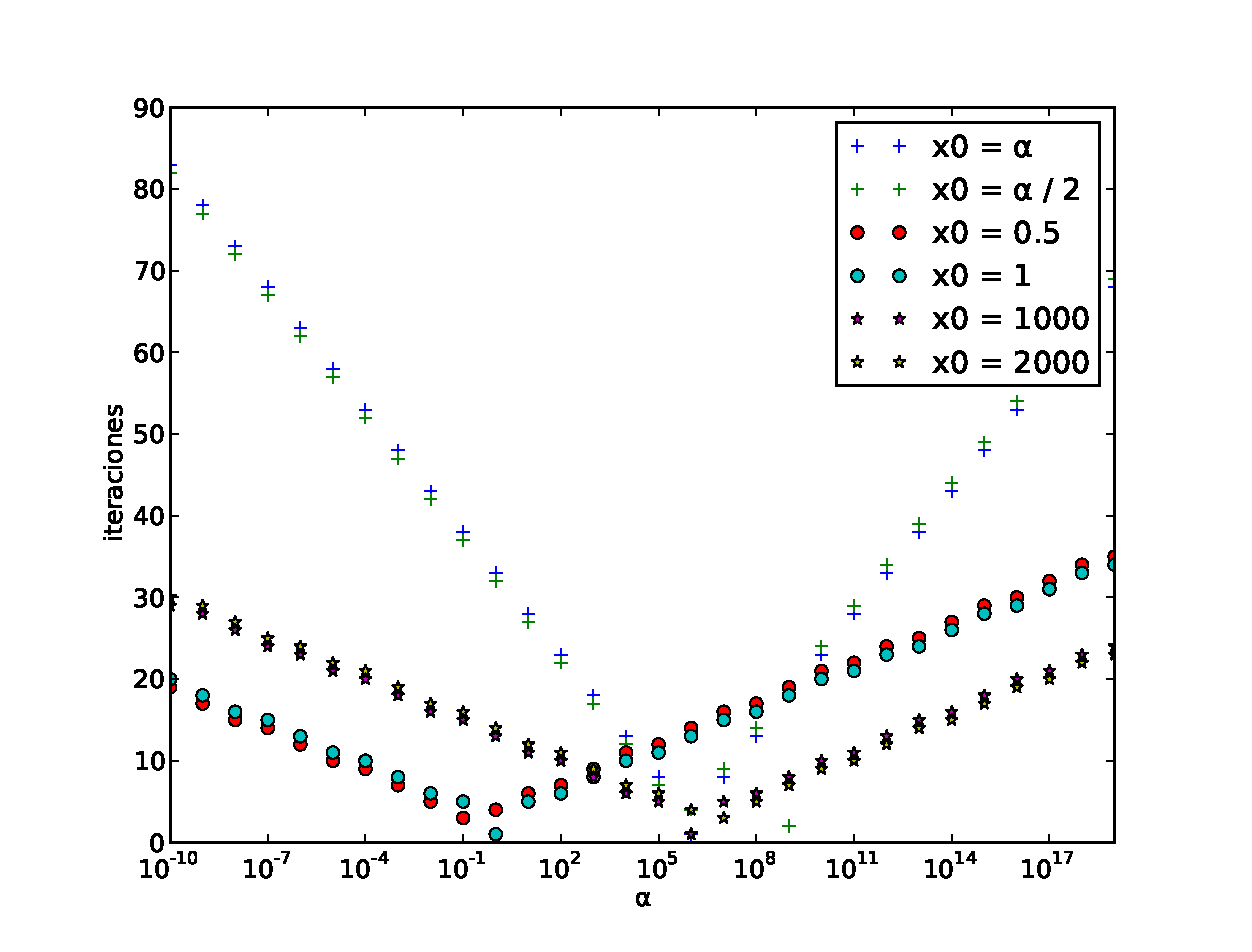
\includegraphics[scale=0.5]{graficos/new/f_newton_x0_fijo_2.eps}
    \caption{\label{fig:f_newton_x0_fijo_2} Gráfico de cantidad de iteraciones fijando $x_0$ variando $\alpha$ para $f(x)$ utilizando el método de Newton (más variantes).}
  \end{center}
\end{figure}

En la Figura~\ref{fig:f_newton_x0_fijo_2} graficamos algunos valores más para
$x_0$ variando las constantes utilizadas. Se observa claramente que variar la
constante produce un \emph{corrimiento} de la cantidad de iteraciones lo cual
tiene sentido ya que se empieza cerca del resultado para diferentes valores de
$\alpha$. Este corrimiento se realiza en base a la magnitud (o valores relativos)
de $x_0$ y no en base a su valor, lo que implica que el corrimiento entre $x_0
= 0.5$ y $x_0 = 1$ es similar al corrimiento entre $x_0 = 1000$ y $x_0 = 2000$
ya que diferencia relativa entre estos valores es de $1/2$.

Se puede observar también que tomando diferentes $x_0$ en relación lineal con
$\alpha$ también produce un corrimiento y no una diferencia en la pendiente.

En base a estos resultados decidimos tomar $x_0 = 1$ para calcular $f(x)$
utilizando el método de Newton ya que mantiene un equilibrio entre magnitudes
muy grandes y magnitudes muy pequeñas.

\subsubsection{Ajuste de $x_0$ para $e(x)$ y el método de Newton}
\label{ssub:ajuste_e_x0_newton}

A diferencia de $f(x)$ para el método de Newton, no contamos con seguridad en
la convergencia de este método para esta función. En las figuras que mostramos
a continuación sólo graficamos los valores para los cuales el método converge
en una cantidad acotada de iteraciones, por esto se verán sectores de cada
variante no graficados.

\begin{figure}[!htbp]
  \begin{center}
    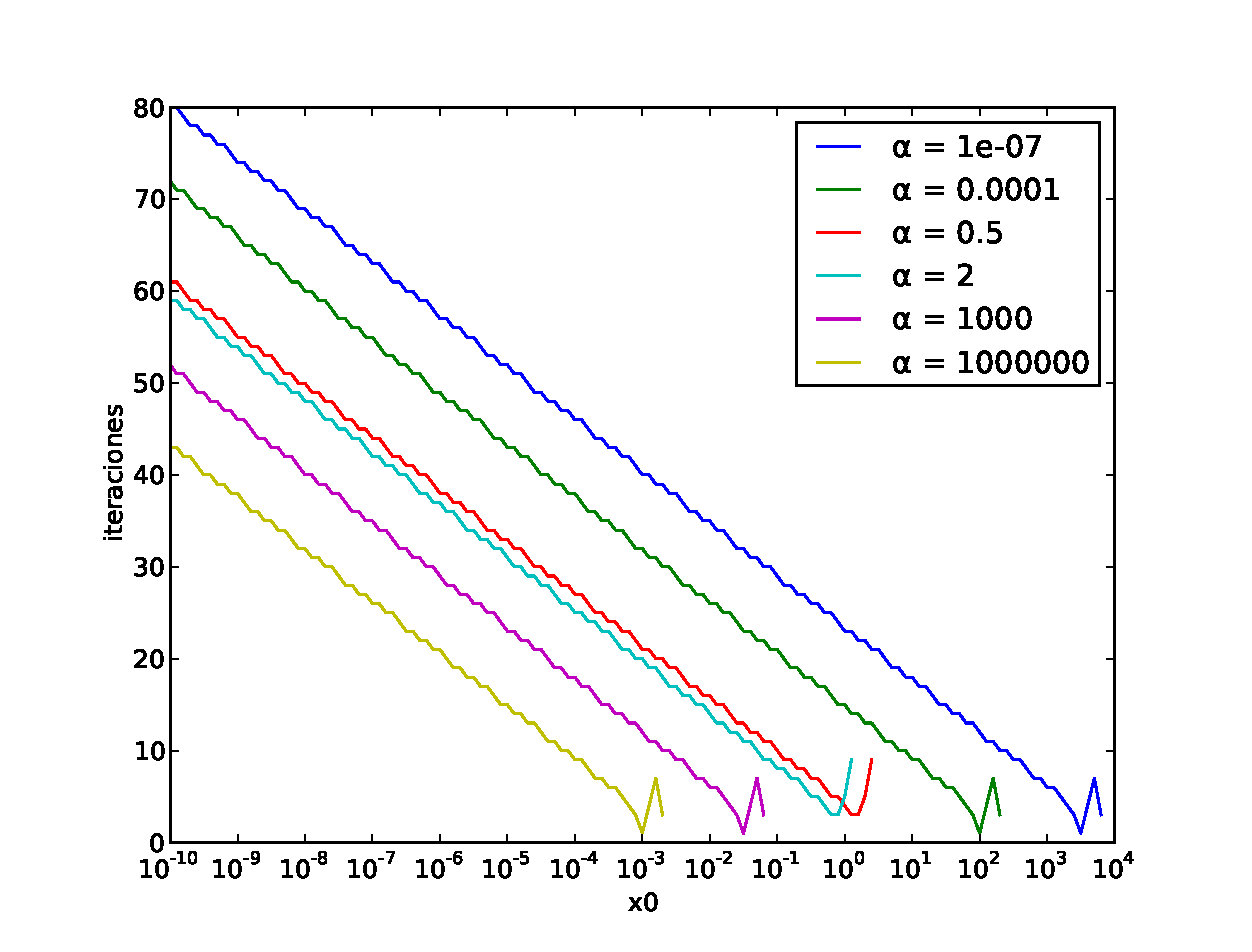
\includegraphics[scale=0.5]{graficos/new/e_newton_x0_variable.eps}
    \caption{\label{fig:e_newton_x0_variable} Gráfico de cantidad de iteraciones fijando $\alpha$ variando $x_0$ para $e(x)$ utilizando el método de Newton.}
  \end{center}
\end{figure}

En la Figura~\ref{fig:e_newton_x0_variable} lo primero que podemos observar es que
como habíamos pensado no todos los $\alpha$ convergen para todos los $x_0$. Cuanto
mayor es el $\alpha$ necesitamos un mayor $x_0$ para lograr la convergencia. No
obstante, si fijamos un $x_0$ constante muy grande, la cantidad de iteraciones
necesarias para llegar al resultado para $\alpha$ chicos es muy grande.

Se nos ocurren dos alternativas posibles del porqué no converge hacia el
resultado. La primera es que simplemente el método no converge para todos los
$x_0$ para todos los $\alpha$ ya que no tenemos un análisis que lo garantice.
La segunda alternativa es que al poseer dos asíntotas, al variar poco algunos
números varía mucho hacia números \textbf{muy} grandes la intersección con las
abscisas de las tangentes o la evaluación de $e(x)$ en valores cercanos al $0$.
Esto puede producir la pérdida de dígitos significativos perjudicando la
convergencia. Para muchas de las pruebas que realizamos durante la
implementación obtuvimos valores intermedios donde la representación de doble
punto flotante nativa utilizada llegaba a $\infty$.

\begin{figure}[!htbp]
  \begin{center}
    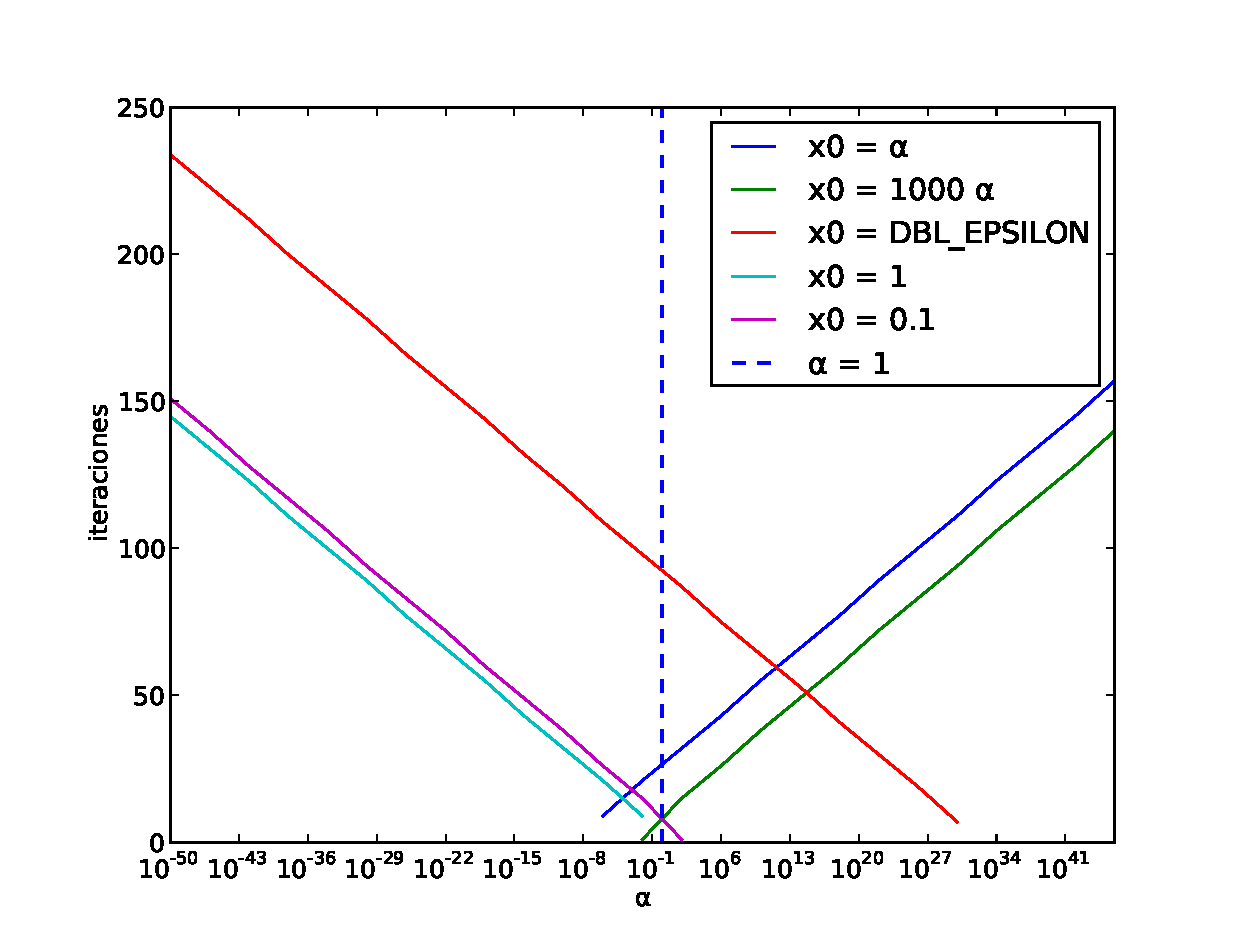
\includegraphics[scale=0.5]{graficos/new/e_newton_x0_fijo.eps}
    \caption{\label{fig:e_newton_x0_fijo} Gráfico de cantidad de iteraciones fijando $x_0$ variando $\alpha$ para $e(x)$ utilizando el método de Newton.}
  \end{center}
\end{figure}

En la Figura~\ref{fig:e_newton_x0_fijo} podemos observar cómo se comporta la
cantidad de iteraciones y la convergencia de diferentes $x_0$ mientras variamos
la magnitud de $\alpha$. Decidimos probar al igual que en el análisis del
método de Newton para $f(x)$ el comportamiento con $x_0 =
\textit{DBL\_EPSILON}$. En este caso, converge para gran cantidad del dominio
pero necesita muchas iteraciones para $\alpha$ pequeños. En el caso de $x_0 =
1 / \alpha$ podemos observar que converge para valores muy grandes de $\alpha$.
Esto se debe a que el punto de inicio se encuentra en la asíntota de las
ordenadas donde la pendiente de la tangente es muy grande, y las sucesivas
iteraciones se mantienen en la misma asíntota mejorando la aproximación en cada
iteración.

Notemos que parecen generar pendientes similares pero invertidas.

Utilizar otras constantes para $x_0$ o multiplicar $\alpha$ por una constante
genera nuevamente un ``corrimiento'' sin cambio perceptible en la pendiente.

Al igual que en el caso anterior decidimos tomar valores para ``equilibrar''
diferentes magnitudes de $\alpha$ alrededor del $1$. Para esto buscamos
mediante una búsqueda binaria (manual) los valores para $x_0$ para producir la
menor cantidad de iteraciones en $\alpha = 1$. Los valores encontrados y que
utilizaremos para $e(x)$ y el método de Newton son:

\[
\begin{cases}
x_0 = 0.1, & \mbox{si } \alpha < 1\\
x_0 = 1 / (\alpha * 10), & \mbox{si } \alpha \ge 1
\end{cases}
\]

La cantidad de iteraciones para estos valores se pueden observar en la
Figura~\ref{fig:e_newton_x0_fijo} donde se encuentra graficada su intersección
en $\alpha = 1$.

\subsubsection{Ajuste de $x_0$ y $x_1$ para $e(x)$ y el método de la Secante}
\label{ssub:ajuste_e_x0_x1_secante}

En el caso del método de la Secante para $e(x)$ debemos elegir tanto $x_0$ como
$x_1$. En esta combinación tampoco tenemos asegurada la convergencia. Al igual
que en el apartado anterior, en las figuras que mostramos a continuación sólo
graficamos los valores para los cuales el método converge.

El enfoque que decidimos tomar para esta combinación es el siguiente: teniendo
en cuenta que el método de la Secante se puede ver como una aproximación por
diferencias finitas del método de Newton, intentamos replicar los resultados,
eligiendo los mismos $x_0$ y ajustando los $x_1$ para obtener valores
similares.

\begin{figure}[!htbp]
  \begin{center}
    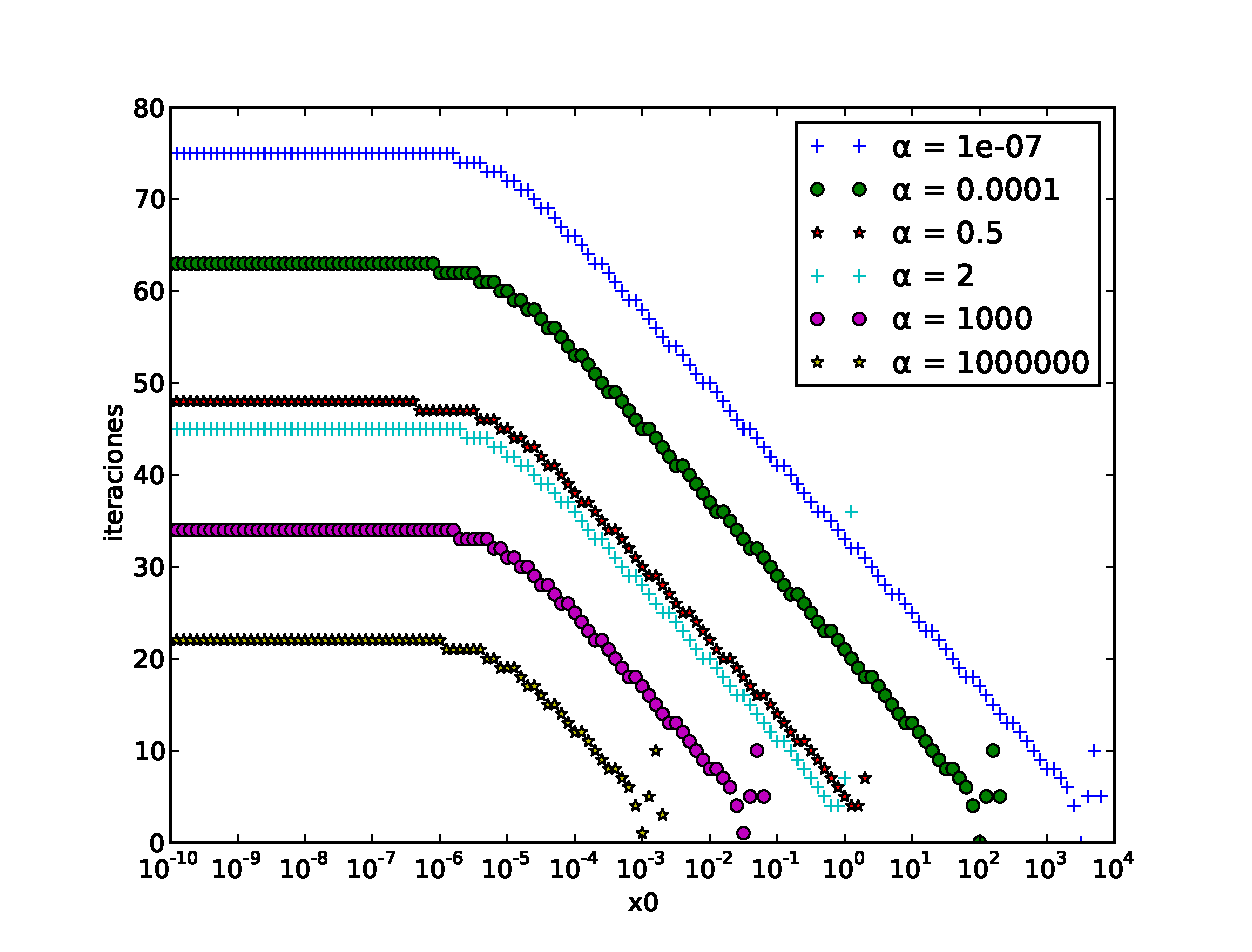
\includegraphics[scale=0.5]{graficos/new/e_secante_x0_variable.eps}
    \caption{\label{fig:e_secante_x0_variable} Gráfico de cantidad de iteraciones fijando $\alpha$ variando $x_0$ para $e(x)$ utilizando el método de la Secante.}
  \end{center}
\end{figure}

En la Figura~\ref{fig:e_secante_x0_variable} podemos observar resultados
similares a los de la Figura~\ref{fig:e_newton_x0_variable}. Al igual que en
esta no todos los $\alpha$ convergen para todos los $x_0$. Las mismas
conclusiones aplican, cuanto mayor es el $\alpha$ necesitamos un mayor $x_0$
para lograr la convergencia a costa de mayor cantidad de iteraciones para
$\alpha$ chicos.

Los $x_1$ tomados para este experimiento son $x_1 = x_0 + 0.0001$. Al elegir
estos $x_1$ cercanos a los $x_0$ la idea fue aproximar la tangente obtenida en
la primera iteración del método de Newton. Puntos $x_1$ más cercanos a $x_0$
producían una menor convergencia en el mismo dominio.

Se puede observar también como la cantidad de iteraciones crece a medida que el
$\alpha$ crece hasta un punto donde la cantidad de iteraciones se mantiene
estable. Creemos que esto se debe a las asíntotas, donde la elección de $x_0$ y
$x_1$ tan grandes producen muy poca variación en el cálculo de la tangente.

Se puede notar también una mayor cantidad de iteraciones necesarias para
alcanzar los mismos resultados que para el método de Newton, lo que concuerda
con el grado de convergencia teórico.

\begin{figure}[!htbp]
  \begin{center}
    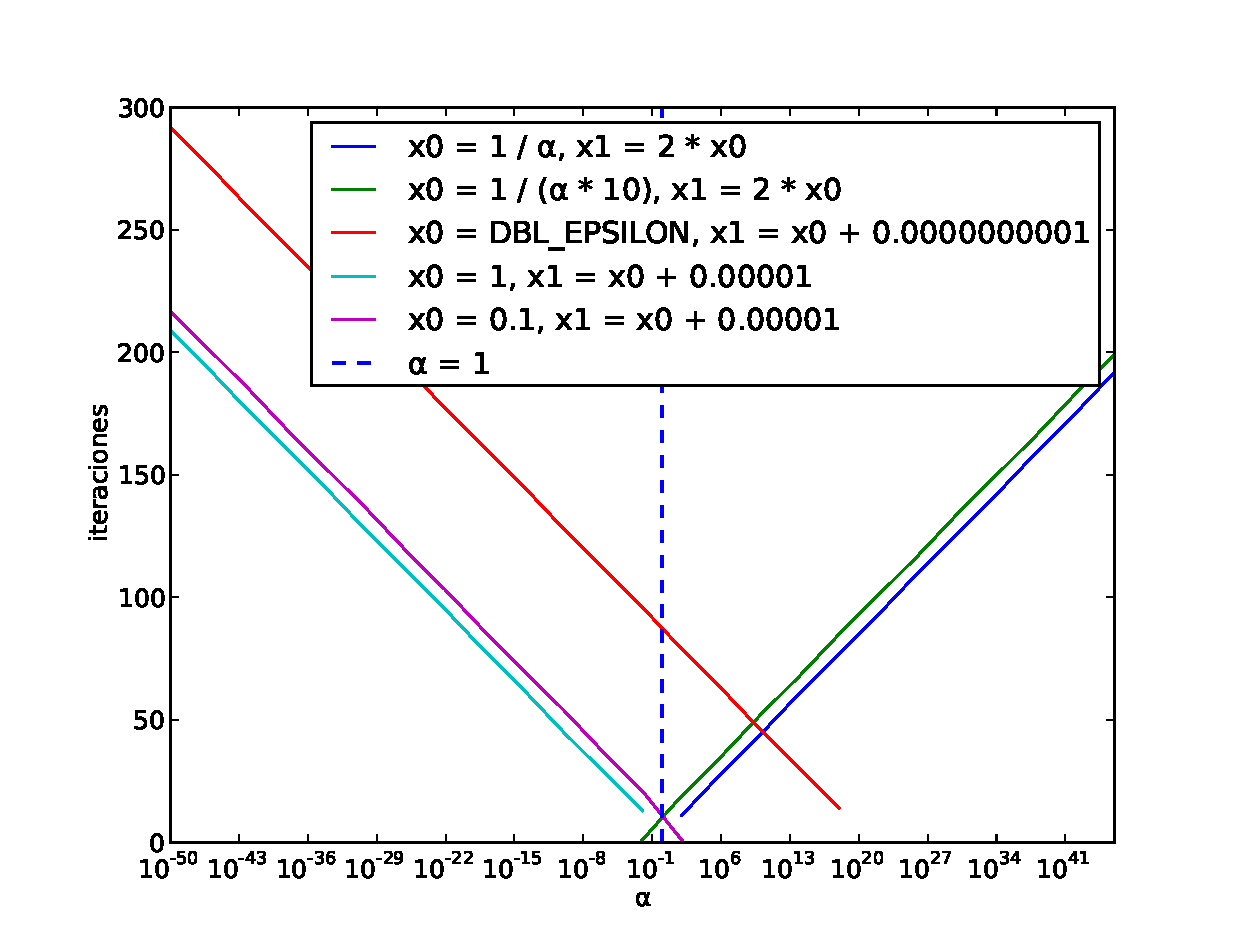
\includegraphics[scale=0.5]{graficos/new/e_secante_x0_fijo.eps}
    \caption{\label{fig:e_secante_x0_fijo} Gráfico de cantidad de iteraciones fijando $x_0$ variando $\alpha$ para $e(x)$ utilizando el método de la Secante.}
  \end{center}
\end{figure}

En la Figura~\ref{fig:e_secante_x0_fijo} podemos observar cómo se comporta la
cantidad de iteraciones y la convergencia de diferentes $x_0$ mientras variamos
la magnitud de $\alpha$. Decidimos probar al igual que en la
Figura~\ref{fig:e_newton_x0_fijo} el comportamiento con $x_0 =
\textit{DBL\_EPSILON}$. Para lograr el mismo dominio de convergencia
necesitamos utilizar un $x_1$ aún más cercano,  $x1 = \textit{DBL\_EPSILON} +
0.0000000001 = x_0 + 0.0000000001$.

Para los casos donde $x_0$ es inverso a $\alpha$ fue necesario multiplicar $x_1
= 2 \times x_0$ para lograr el mismo dominio de convergencia que en el método
de Newton.

Estos resultados mantienen la misma forma que los de la
Figura~\ref{fig:e_newton_x0_fijo}, incluso los valores de $x_0$ se mantienen
para lograr ``equilibrar'' la convergencia en $\alpha = 1$.

Los valores encontrados y que utilizaremos para $e(x)$ y el método de la
Secante son:

\[
\begin{cases}
x_0 = 0.1 \wedge x_1 = x_0 + 0.00001, & \mbox{si } \alpha < 1\\
x_0 = 1 / (\alpha * 10) \wedge x_1 = x_0 * 2, & \mbox{si } \alpha \ge 1
\end{cases}
\]

La cantidad de iteraciones para estos valores se pueden observar en la
Figura~\ref{fig:e_secante_x0_fijo} donde se encuentra graficada su intersección
en $\alpha = 1$.

    \newpage
    \section{Resultados}
% Deben incluir los resultados de los experimentos, utilizando el formato mas
% adecuado para su presentacion. Deberan especicar claramente a que
% experiencia corresponde cada resultado. No se incluiran aqu corridas de
% maquina. Algo fundamental en su aprendizaje en la materia es la presentacion
% de resultados de forma clara y concisa para el lector

\subsection{Hipótesis}
Como vimos en la Introducción Teórica, Newton tiene convergencia cuadrática y Secante $supralineal$ (alrededor de 1.6).\\

Sería normal suponer que Newton tiene mejor performance dado que converge más rápido. Sin embargo para comparar performance, debemos considerar costo como rapidez de convergencia. Un algoritmo que converge rápido pero tarda algunos segundos por iteración podría tomar mas tiempo que uno que converge mas lento pero toma solo algunos milisegundos por iteración.\\

Podemos asumir que el costo de una iteración está marcado por la evaluación de la función, de hecho, este vendría a ser nuestro caso. Entonces la cantidad de evaluaciones de una función puede ser una buena medida de costo.\\

Secante solo requiere una evaluación de la función por iteración, dado que el valor de $f(x_{n - 1})$ se puede guardar de la iteración previa.\\

Newton requiere una evaluación de la función y otra de su derivada por iteración. Es complicado estimar el costo de evaluar la derivada en general. En algunos casos la derivada puede ser fácil de evaluar y en otros puede ser incluso mas difícil de evaluar que la función original.\\

Podemos asumir entonces, que en general, calcular la derivada es al menos tan costoso como calcular la función. Por lo tanto asumimos que Newton va a tomar dos evaluaciones por iteración.\\

Este análisis nos lleva a suponer que Secante debería ser mas performante que Newton en general.

\subsection{Casos de Prueba}
La aproximación inicial que tuvimos fue tomar cada uno de los parámetros, fijar los demás y hacer un análisis de cada uno de los factores de estudio (tiempo, iteraciones, convergencia, etc.) haciendo crecer los parámetros de turno. Claramente la cantidad de casos era mucha y en general los resultados eran difíciles de interpretar y no aportaban al propósito de develar si nuestra hipótesis se cumplía.\\

Por lo tanto decidimos que lo mejor sería solamente tomar un par de combinaciones de todas las posibles que nos parecieran que fueran representativas. En nuestro caso al ya tener $x_0$ y $x_1$ definidos en base a previa experimentación decidimos hacer comparaciones entre los métodos en términos de iteraciones y tiempo de ejecución para $\alpha$'s crecientes.\\

\subsubsection{Iteraciones} % (fold)
\label{ssub:iteraciones}

En el caso de hacer crecer $\alpha$ para ver cómo se comportan en función de las iteraciones, nuestra suposición es que Newton tomará menos iteraciones que Secante. Ahora, para Newton con $f(x)$ y $e(x)$ suponemos que el primero tomará menos iteraciones ya que el segundo cuenta con un cociente extra para calcular con respecto al primero en cada iteración.\\

\begin{figure}[!htbp]
  \begin{center}
    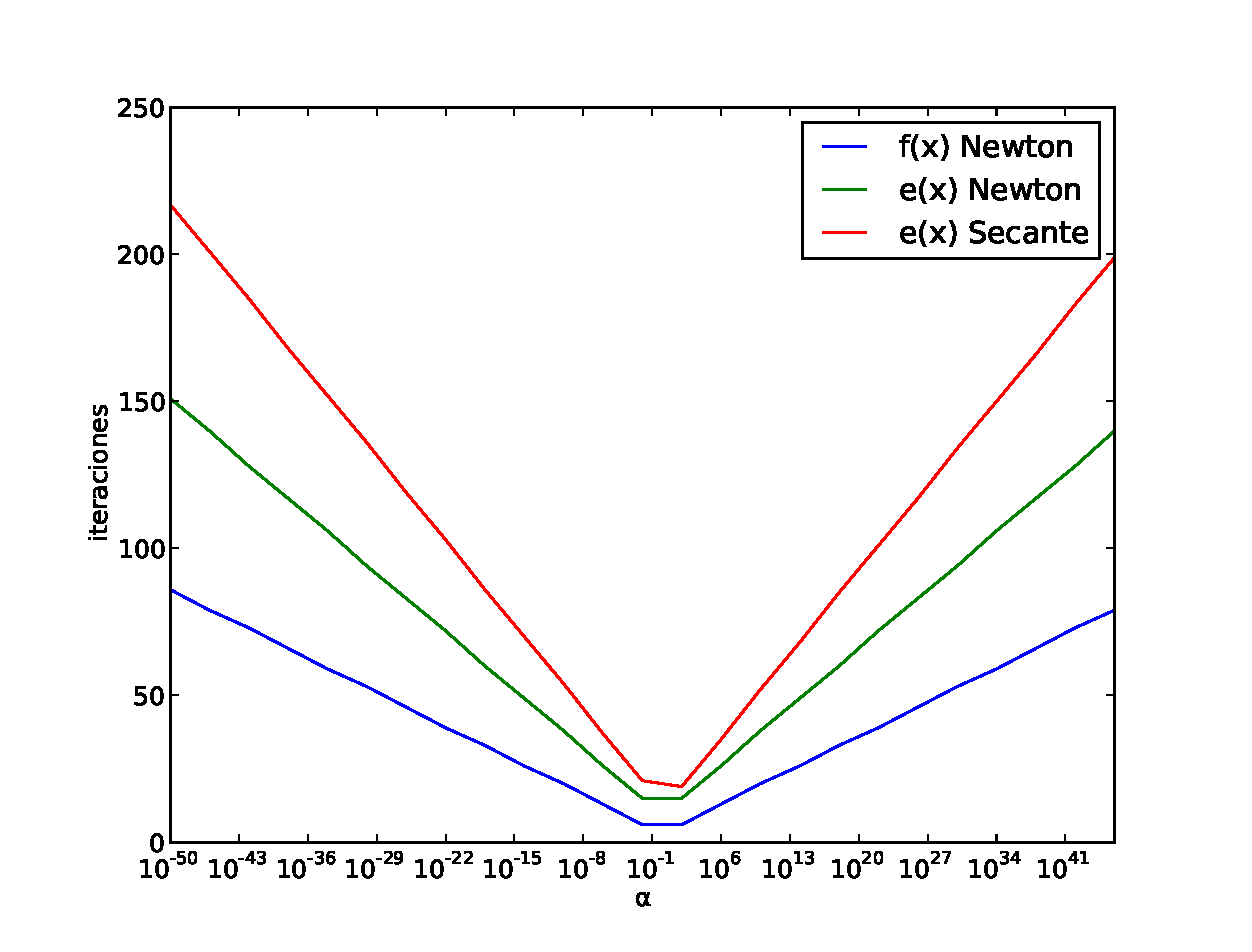
\includegraphics[scale=0.5]{graficos/new/comparacion_iteraciones.eps}
    \caption{\label{fig:comparacion_iteraciones} Gráfico comparativo de $\alpha$ en función de la cantidad de iteraciones}
  \end{center}
\end{figure}

Como podemos ver en la Figura~\ref{fig:comparacion_iteraciones} nuestras expectactivas se cumplieron, y podemos ver además como las iteraciones disminuyen a medida que los puntos iniciales están cerca del $\alpha$.

% subsubsection iteraciones (end)

\subsubsection{Tiempo de Ejecución} % (fold)
\label{ssub:tiempo_de_ejecuci_n}

En esta sección entra en juego lo que hablamos en la parte de Hipótesis. En términos prácticos, uno de los factores a tomar en cuenta es cuán rápido obtenemos el resultado requerido. Como bien enunciamos anteriormente suponemos que Secante será mas rápido que Newton.\\

\begin{figure}[!htbp]
  \begin{center}
    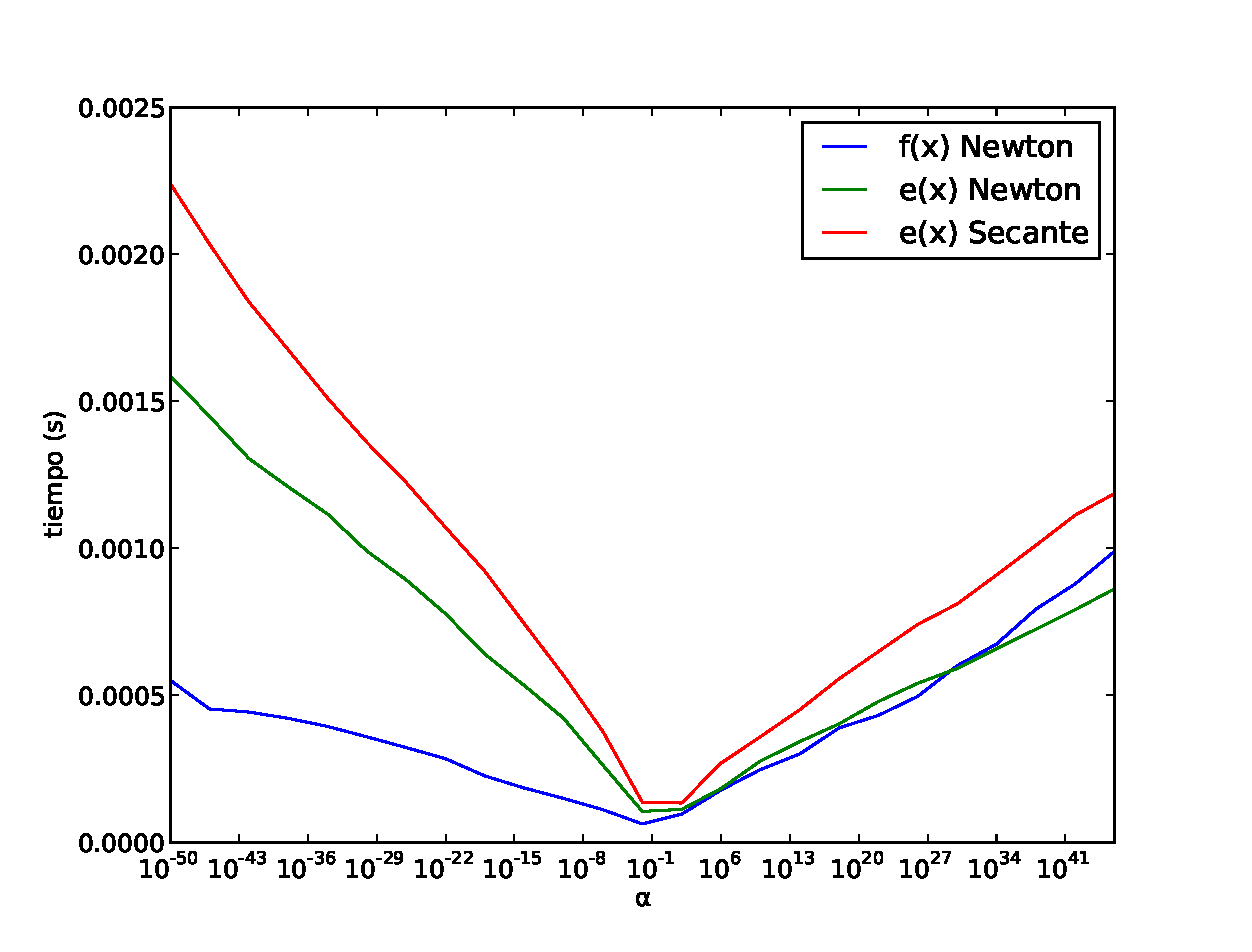
\includegraphics[scale=0.5]{graficos/new/comparacion_tiempos.eps}
    \caption{\label{fig:comparacion_tiempos} Gráfico comparativo de $\alpha$ en función del tiempo de ejecución}
  \end{center}
\end{figure}

En la Figura~\ref{fig:comparacion_tiempos} vemos cómo lo que habíamos anticipado al final no sucede, Newton con $f(x)$ es el que termina siendo mas performante y lo otro que podemos ver es que para $e(x)$ con Newton y Secante, el primero es mas performante desde valores chicos, pasando por el valor exacto, hasta que cuando $alpha$ crece mas, llega un punto donde Newton supera a Secante.\\

% subsubsection tiempo_de_ejecuci_n (end)
    \newpage
    \section{Discusión y Conclusiones}
% Se incluira aqu un analisis de los resultados obtenidos en la seccion
% anterior (se analizara su validez, coherencia, etc.). Deben analizarse como
% materianimo los lostems pedidos en el enunciado. No es aceptable decir que
% \los resultados fueron los esperados", sin hacer clara referencia a la
% teoremasa a la cual se ajustan. Ademas, se deben mencionar los resul- tados
% interesantes y los casos \patologicos" encontrados.

\subsection{Casos intersantes}

primer caso
===========

bin/tp1 0.0000000000000000000000000000000001 e n r 0.000000000000000000000000000001 1 2
se queda saltando entre dos numeros diferentes

con numeros tan chicos de alhpa el punto flotante explota y se pone a hacer cosas raras, analizarlo un poco mas y decir por que parece que hace esto.


segundo caso
============

una corrida, si le agregamos un 0 al error relativo corta por cantidad de iteraciones y no por llegar al error relativo

*********************** bin/tp1 9999 e s r 0.000000000000001 0.09999 0.009999
Buscando 1 / sqrt(9999.000000)
Utilizando e(x)
Utilizando Secante
Criterio de parada error relativo con limite 0.000000
Utilizando x0=0.099990 y x1=0.009999

0.010026267273090912895971982266019040253013372421264648437500000000000000000000000000000000000000000 Iter
0.010000505837327295852179354085365048376843333244323730468750000000000000000000000000000000000000000 Iter
0.010000500015077814705555248053769901162013411521911621093750000000000000000000000000000000000000000 Iter
0.010000500037503143660466697895117249572649598121643066406250000000000000000000000000000000000000000 Iter
0.010000500037503126313231938127046305453404784202575683593750000000000000000000000000000000000000000 Iter

0.010000500037503126313231938127046305453404784202575683593750000000000000000000000000000000000000000 resultado
5 iteraciones
-0.000000000001818989403545856475830078125000000000000000000000000000000000000000000000000000000000000 error absoluto
-0.000000000000000181917132067792432769858681142675088907883197372229722166281362660811282694339752197 error relativo
0.000067999999999999999463970445923166607826715335249900817871093750000000000000000000000000000000000 tiempo

*********************** bin/tp1 9999 e s r 0.0000000000000001 0.09999 0.009999
0.010000500037503124578508462150239211041480302810668945312500000000000000000000000000000000000000000 Iter
0.010000500037503124578508462150239211041480302810668945312500000000000000000000000000000000000000000 Iter
0.010000500037503124578508462150239211041480302810668945312500000000000000000000000000000000000000000 Iter
0.010000500037503124578508462150239211041480302810668945312500000000000000000000000000000000000000000 Iter
0.010000500037503124578508462150239211041480302810668945312500000000000000000000000000000000000000000 Iter
0.010000500037503124578508462150239211041480302810668945312500000000000000000000000000000000000000000 Iter

0.010000500037503124578508462150239211041480302810668945312500000000000000000000000000000000000000000 resultado
1000 iteraciones
0.000000000001818989403545856475830078125000000000000000000000000000000000000000000000000000000000000 error absoluto
0.000000000000000181917132067792432769858681142675088907883197372229722166281362660811282694339752197 error relativo
0.011587999999999999342636947119444812415167689323425292968750000000000000000000000000000000000000000 tiempo

todo depende, de que depende? de si buscas velocidad o precision
Veamos lo que podemos implicar a partir de la comparación que se hizo de cada gráfico
\begin{itemize}
\item {\bf Cantidad de iteraciones f(x) con Newton y Secante:} Acá se puede observar que a medida que el $x_0$ crece la cantidad de iteraciones crece pero mas despacio, casi logrando un crecimiento logarítmico. Sin embargo es apreciable que el método de Newton toma menos iteraciones.
\item {\bf Error Absoluto f(x) con Newton y Secante:} En los gráficos se puede apreciar que cuando $x_0$ es chico Newton y Secante alcanzan el criterio de parada casi en los mismos puntos. Pero a medida que $x_0$ crece Secante empieza a llegar antes al criterio de parada. Se podría decir que Secante es mas preciso que Newton.
\item {\bf Tiempo de Computo f(x) con Newton y Secante:} En este caso es claro ver  

\end{itemize}




    \newpage
    \section{Conclusiones}
% Esta seccion debe contener las conclusiones generales del trabajo. Se deben
% mencionar las relaciones de la discusion sobre las que se tiene certeza,
% junto con comentarios y observaciones generales aplicables a todo el proceso.
% Mencionar tambien posibles extensiones a los metodos, experimentos que hayan
% quedado pendientes, etc
todo depende, de que depende? de si buscas velocidad o precision
Veamos lo que podemos implicar a partir de la comparación que se hizo de cada gráfico
\begin{itemize}
\item {\bf Cantidad de iteraciones f(x) con Newton y Secante:} Acá se puede observar que a medida que el $x_0$ crece la cantidad de iteraciones crece pero mas despacio, casi logrando un crecimiento logarítmico. Sin embargo es apreciable que el método de Newton toma menos iteraciones.
\item {\bf Error Absoluto f(x) con Newton y Secante:} En los gráficos se puede apreciar que cuando $x_0$ es chico Newton y Secante alcanzan el criterio de parada casi en los mismos puntos. Pero a medida que $x_0$ crece Secante empieza a llegar antes al criterio de parada. Se podría decir que Secante es mas preciso que Newton.
\item {\bf Tiempo de Computo f(x) con Newton y Secante:} En este caso es claro ver  

\end{itemize}




    \newpage

    \appendix
% En el apendice A se incluira el enunciado del TP. En el apendice B se
% incluiran los codigos fuente de las funciones relevantes desde el punto de
% vista numerico. Resultados que valga la pena mencionar en el trabajo pero que
% sean demasiado especicos para aparecer en el cuerpo principal del trabajo
% podran mencionarse en sucesivos apendices rotulados con las letras mayusculas
% del alfabeto romano. Por ejemplo: la demostracion de una propiedad que
% aplican para optimizar el algoritmo que programaron para resolver un
% problema.
%    \begin{center}
\begin{tabular}{r|cr}
 \begin{tabular}{c}
{\large\bf\textsf{\ M\'etodos Num\'ericos\ }}\\ 
Segundo Cuatrimestre 2013\\
{\bf Trabajo Pr\'actico 1}
\end{tabular} &
\begin{tabular}{@{} p{1.6cm} @{}}
\includegraphics[width=1.6cm]{../../logodpt.jpg}
\end{tabular} &
\begin{tabular}{l @{}}
 \emph{Departamento de Computaci\'on} \\
 \emph{Facultad de Ciencias Exactas y Naturales} \\
 \emph{Universidad de Buenos Aires} \\
\end{tabular} 
\end{tabular}
\end{center}

\vskip 25pt
\hrule
\vskip 11pt
 
\textbf{Introducci\'on}

En las \'ultimas dos d\'ecadas se han producido avances muy significativos en el \'area de Computaci\'on Gr\'afica, en
particular en el desarrollo de animaciones y video juegos en 3D donde se obtienen resultados muy detallados y con un
alto nivel de realismo. 

Un aspecto importante que contribuye en este sentido es la iluminaci\'on de la escena y el reflejo de la luz en los
objetos o personajes de la misma. A grandes rasgos, el manejo de la iluminaci\'on se hace de la siguiente forma. Dada
una superficie en el espacio, se calculan los vectores normales a la misma (recordar \emph{An\'alisis II}) sobre un
conjunto determinado de puntos y luego estos vectores son utilizados, en conjunto con el modelo de iluminaci\'on, para
calcular su color final y la interacci\'on con otras superficies. Adem\'as, por cuestiones pr\'acticas, los vectores
normales deber ser almacenados como vectores unitarios, es decir, que su norma Euclideana ($\|~\|_2$) sea 1.

Dado un vector $y \in \mathbb{R}^3$ cualquiera, podemos convertirlo en uno unitario dividi\'endolo por $\|y\|_2$, es
decir, 
\begin{eqnarray*}
\| y \|_2 & = & \sqrt{y_1^2 + y_2^2 + y_3^2}\\
z & = & \frac{y}{\|y\|_2}.
\end{eqnarray*}
\noindent Durante la ejecuci\'on del programa, esta operaci\'on es realizada millones de veces por segundo, por lo cual
es importante realizarla en el menor tiempo posible, eventualmente resignando precisi\'on en el
resultado. Dado el contexto, peque\~nas reducciones en el tiempo de ejecuci\'on pueden mejorar considerablemente el
comportamiento general.

\textbf{El problema}

Sean $y = (y_1, y_2, y_3) \in \mathbb{R}^3$ un vector gen\'erico y $\alpha = y_1^2 + y_2^2 + y_3^2$. El problema de
obtener un vector unitario que posea la misma direcci\'on que $y$ lo podemos plantear como multiplicarlo por
$1/\sqrt{\alpha}$. Luego, el problema de normalizar un vector radica principalmente en el c\'alculo de este valor, que
involucra una divisi\'on y el c\'alculo de una ra\'iz cuadrada. 

Sin utilizar funciones ya provistas por el lenguaje de programaci\'on a utilizar, el c\'alculo de $1/\sqrt{\alpha}$ se
pueden formular como un problema de b\'usqueda de ceros de una funci\'on de (al menos) las siguientes dos formas:
\begin{itemize}
\item Aproximar $\beta = \sqrt{\alpha}$ como un cero de $f(x) = x^2 - \alpha$, y luego realizar $1/\beta$. 
\item Definir la funci\'on $e(x) = \frac{1}{x^2} - \alpha$, que permite calcular el error de una aproximaci\'on de
$1/\sqrt{\alpha}$. En particular, uno de los ceros de esta funci\'on es el valor buscado.
\end{itemize}

Estas dos reformulaciones del problema nos permiten atacarlo con m\'etodos de b\'usqueda de ceros de funciones en una
variable.

\textbf{Enunciado}

El objetivo del trabajo pr\'actico consiste en implementar un programa que permita calcular, dado $\alpha \in
\mathbb{R}$, $1/\sqrt{\alpha}$. Para ello, se deber\'a considerar las funciones $f(x)$ y $e(x)$ definidas
anteriormente, distintos m\'etodos vistos en clase que permitan resolver el problema planteado y realizar un an\'alisis
completo del comportamiento de los mismos. 

Los requisitos m\'inimos a cumplir son los siguientes:

\begin{itemize}
\item Implementar el m\'etodo de Newton para la funci\'on $f(x)$. Incluir en el informe la demostraci\'on de
convergencia (Ejercicio 3, Pr\'actica 1). Para la funci\'on $e(x)$, implementar al menos dos m\'etodos (uno de los
cuales debe ser el de Newton).   
\item Para cada m\'etodo, estudiar experimentalmente la convergencia, tiempo de ejecuci\'on, cantidad de iteraciones,
criterios de parada, precisi\'on en el resultado, y cualquier otro par\'ametro que considere necesario evaluar. Realizar experimentos
computacionales considerando un rango amplio de valores posibles para $\alpha$ y distintos puntos iniciales
para los m\'etodos. Analizar y justificar detalladamente los resultados obtenidos.
\item Una vez fijados los mejores par\'ametros para cada m\'etodo, realizar una comparaci\'on entre las tres formas
alternativas de resolver el problema (Newton para $f(x)$, y Newton m\'as el otro m\'etodo para $e(x)$) en t\'erminos de
tiempo de ejecuci\'on, precisi\'on en la soluci\'on, cantidad de iteraciones, etc. Determinar experimentalmente que
variante seleccionar\'ia para su utilizaci\'on en la pr\'actica.
\end{itemize}

\vskip 15pt

\hrule

\vskip 11pt


{\bf \underline{Fechas de entrega}}
\begin{itemize}
 \item \emph{Formato Electr\'onico:} Domingo 1° de Septiembre de 2013, hasta las 23:59 hs, enviando el trabajo (informe +
 c\'odigo) a la direcci\'on \verb+metnum.lab@gmail.com+. El subject del email debe comenzar con el texto \verb+[TP1]+
 seguido de la lista de apellidos  de los integrantes del grupo.
 \item \emph{Formato f\'isico:} Lunes 2 de Septiembre de 2013, de 17 a 18 hs.
\end{itemize}

\noindent \textbf{Importante:} El horario es estricto. Los correos recibidos despu\'es de la hora indicada ser\'an considerados re-entrega.
    \section{Referencias}
% Es importante incluir referencias a libros, articleculos y paginas de
% Internet consultados durante el desarrollo del trabajo, haciendo referencia a
% estos materiales a lo largo del informe. Se deben citar tambien las
% comunicaciones personales con otros grupos

\begin{itemize}

    \item Numerical Analysis, Richard L. Burden, John Douglas Faires. Cengage Learning, 2005.

\end{itemize}

    \section{Anexos}
% \subsection{Pseudocodigo de metodos}
% copiar pseudocodigo (comentarios) de %newton_start newton_iter secante_start
% %secante_iter y loop principal

% \subsection{Detalle de experimentos}

% en este anexo detallamos los diferentes experimentos, como replicarlos y la
% motivacion detras de cada uno de ellos.

% por cada experimento indicar en que archivo esta, y que corridas se hicieron
% con que datos y por que elegimos hacer ese exp.
\begin{center}
\begin{tabular}{r|cr}
 \begin{tabular}{c}
{\large\bf\textsf{\ M\'etodos Num\'ericos\ }}\\ 
Segundo Cuatrimestre 2013\\
{\bf Trabajo Pr\'actico 1}
\end{tabular} &
% \begin{tabular}{@{} p{1.6cm} @{}}
% \includegraphics[width=1.6cm]{../../logodpt.jpg}
% \end{tabular} &
\begin{tabular}{l @{}}
 \emph{Departamento de Computaci\'on} \\
 \emph{Facultad de Ciencias Exactas y Naturales} \\
 \emph{Universidad de Buenos Aires} \\
\end{tabular} 
\end{tabular}
\end{center}

\vskip 25pt
\hrule
\vskip 11pt
 
\textbf{Introducci\'on}

En las \'ultimas dos d\'ecadas se han producido avances muy significativos en el \'area de Computaci\'on Gr\'afica, en
particular en el desarrollo de animaciones y video juegos en 3D donde se obtienen resultados muy detallados y con un
alto nivel de realismo. 

Un aspecto importante que contribuye en este sentido es la iluminaci\'on de la escena y el reflejo de la luz en los
objetos o personajes de la misma. A grandes rasgos, el manejo de la iluminaci\'on se hace de la siguiente forma. Dada
una superficie en el espacio, se calculan los vectores normales a la misma (recordar \emph{An\'alisis II}) sobre un
conjunto determinado de puntos y luego estos vectores son utilizados, en conjunto con el modelo de iluminaci\'on, para
calcular su color final y la interacci\'on con otras superficies. Adem\'as, por cuestiones pr\'acticas, los vectores
normales deber ser almacenados como vectores unitarios, es decir, que su norma Euclideana ($\|~\|_2$) sea 1.

Dado un vector $y \in \mathbb{R}^3$ cualquiera, podemos convertirlo en uno unitario dividi\'endolo por $\|y\|_2$, es
decir, 
\begin{eqnarray*}
\| y \|_2 & = & \sqrt{y_1^2 + y_2^2 + y_3^2}\\
z & = & \frac{y}{\|y\|_2}.
\end{eqnarray*}
\noindent Durante la ejecuci\'on del programa, esta operaci\'on es realizada millones de veces por segundo, por lo cual
es importante realizarla en el menor tiempo posible, eventualmente resignando precisi\'on en el
resultado. Dado el contexto, peque\~nas reducciones en el tiempo de ejecuci\'on pueden mejorar considerablemente el
comportamiento general.

\textbf{El problema}

Sean $y = (y_1, y_2, y_3) \in \mathbb{R}^3$ un vector gen\'erico y $\alpha = y_1^2 + y_2^2 + y_3^2$. El problema de
obtener un vector unitario que posea la misma direcci\'on que $y$ lo podemos plantear como multiplicarlo por
$1/\sqrt{\alpha}$. Luego, el problema de normalizar un vector radica principalmente en el c\'alculo de este valor, que
involucra una divisi\'on y el c\'alculo de una ra\'iz cuadrada. 

Sin utilizar funciones ya provistas por el lenguaje de programaci\'on a utilizar, el c\'alculo de $1/\sqrt{\alpha}$ se
pueden formular como un problema de b\'usqueda de ceros de una funci\'on de (al menos) las siguientes dos formas:
\begin{itemize}
\item Aproximar $\beta = \sqrt{\alpha}$ como un cero de $f(x) = x^2 - \alpha$, y luego realizar $1/\beta$. 
\item Definir la funci\'on $e(x) = \frac{1}{x^2} - \alpha$, que permite calcular el error de una aproximaci\'on de
$1/\sqrt{\alpha}$. En particular, uno de los ceros de esta funci\'on es el valor buscado.
\end{itemize}

Estas dos reformulaciones del problema nos permiten atacarlo con m\'etodos de b\'usqueda de ceros de funciones en una
variable.

\textbf{Enunciado}

El objetivo del trabajo pr\'actico consiste en implementar un programa que permita calcular, dado $\alpha \in
\mathbb{R}$, $1/\sqrt{\alpha}$. Para ello, se deber\'a considerar las funciones $f(x)$ y $e(x)$ definidas
anteriormente, distintos m\'etodos vistos en clase que permitan resolver el problema planteado y realizar un an\'alisis
completo del comportamiento de los mismos. 

Los requisitos m\'inimos a cumplir son los siguientes:

\begin{itemize}
\item Implementar el m\'etodo de Newton para la funci\'on $f(x)$. Incluir en el informe la demostraci\'on de
convergencia (Ejercicio 3, Pr\'actica 1). Para la funci\'on $e(x)$, implementar al menos dos m\'etodos (uno de los
cuales debe ser el de Newton).   
\item Para cada m\'etodo, estudiar experimentalmente la convergencia, tiempo de ejecuci\'on, cantidad de iteraciones,
criterios de parada, precisi\'on en el resultado, y cualquier otro par\'ametro que considere necesario evaluar. Realizar experimentos
computacionales considerando un rango amplio de valores posibles para $\alpha$ y distintos puntos iniciales
para los m\'etodos. Analizar y justificar detalladamente los resultados obtenidos.
\item Una vez fijados los mejores par\'ametros para cada m\'etodo, realizar una comparaci\'on entre las tres formas
alternativas de resolver el problema (Newton para $f(x)$, y Newton m\'as el otro m\'etodo para $e(x)$) en t\'erminos de
tiempo de ejecuci\'on, precisi\'on en la soluci\'on, cantidad de iteraciones, etc. Determinar experimentalmente que
variante seleccionar\'ia para su utilizaci\'on en la pr\'actica.
\end{itemize}


\end{document}
